\documentclass[journal,12pt,twocolumn]{IEEEtran}

\usepackage{setspace}
\usepackage{gensymb}
\singlespacing
\usepackage[cmex10]{amsmath}

\usepackage{amsthm}

\usepackage{mathrsfs}
\usepackage{txfonts}
\usepackage{stfloats}
\usepackage{bm}
\usepackage{cite}
\usepackage{cases}
\usepackage{subfig}

\usepackage{longtable}
\usepackage{multirow}

\usepackage{enumitem}
\usepackage{mathtools}
\usepackage{steinmetz}
\usepackage{tikz}
\usepackage{circuitikz}
\usepackage{verbatim}
\usepackage{tfrupee}
\usepackage[breaklinks=true]{hyperref}
\usepackage{graphicx}
\usepackage{tkz-euclide}

\usetikzlibrary{calc,math}
\usepackage{listings}
    \usepackage{color}                                            %%
    \usepackage{array}                                            %%
    \usepackage{longtable}                                        %%
    \usepackage{calc}                                             %%
    \usepackage{multirow}                                         %%
    \usepackage{hhline}                                           %%
    \usepackage{ifthen}                                           %%
    \usepackage{lscape}     
\usepackage{multicol}
\usepackage{chngcntr}

\DeclareMathOperator*{\Res}{Res}

\renewcommand\thesection{\arabic{section}}
\renewcommand\thesubsection{\thesection.\arabic{subsection}}
\renewcommand\thesubsubsection{\thesubsection.\arabic{subsubsection}}

\renewcommand\thesectiondis{\arabic{section}}
\renewcommand\thesubsectiondis{\thesectiondis.\arabic{subsection}}
\renewcommand\thesubsubsectiondis{\thesubsectiondis.\arabic{subsubsection}}


\hyphenation{op-tical net-works semi-conduc-tor}
\def\inputGnumericTable{}                                 %%

\newcommand{\permcomb}[4][0mu]{{{}^{#3}\mkern#1#2_{#4}}}
\newcommand{\perm}[1][-3mu]{\permcomb[#1]{P}}
\newcommand*{\comb}[1][-1mu]{\permcomb[#1]{C}}

\lstset{
%language=C,
frame=single, 
breaklines=true,
columns=fullflexible
}
\begin{document}

\newcommand{\BEQA}{\begin{eqnarray}}
\newcommand{\EEQA}{\end{eqnarray}}
\newcommand{\define}{\stackrel{\triangle}{=}}
\bibliographystyle{IEEEtran}
\raggedbottom
\setlength{\parindent}{0pt}
\providecommand{\mbf}{\mathbf}
\providecommand{\pr}[1]{\ensuremath{\Pr\left(#1\right)}}
\providecommand{\qfunc}[1]{\ensuremath{Q\left(#1\right)}}
\providecommand{\sbrak}[1]{\ensuremath{{}\left[#1\right]}}
\providecommand{\lsbrak}[1]{\ensuremath{{}\left[#1\right.}}
\providecommand{\rsbrak}[1]{\ensuremath{{}\left.#1\right]}}
\providecommand{\brak}[1]{\ensuremath{\left(#1\right)}}
\providecommand{\lbrak}[1]{\ensuremath{\left(#1\right.}}
\providecommand{\rbrak}[1]{\ensuremath{\left.#1\right)}}
\providecommand{\cbrak}[1]{\ensuremath{\left\{#1\right\}}}
\providecommand{\lcbrak}[1]{\ensuremath{\left\{#1\right.}}
\providecommand{\rcbrak}[1]{\ensuremath{\left.#1\right\}}}
\theoremstyle{remark}
\newtheorem{rem}{Remark}
\newcommand{\sgn}{\mathop{\mathrm{sgn}}}
\providecommand{\abs}[1]{\vert#1\vert}
\providecommand{\res}[1]{\Res\displaylimits_{#1}} 
\providecommand{\norm}[1]{\lVert#1\rVert}
%\providecommand{\norm}[1]{\lVert#1\rVert}
\providecommand{\mtx}[1]{\mathbf{#1}}
\providecommand{\mean}[1]{E[ #1 ]}
\providecommand{\fourier}{\overset{\mathcal{F}}{ \rightleftharpoons}}
%\providecommand{\hilbert}{\overset{\mathcal{H}}{ \rightleftharpoons}}
\providecommand{\system}{\overset{\mathcal{H}}{ \longleftrightarrow}}
	%\newcommand{\solution}[2]{\textbf{Solution:}{#1}}
\newcommand{\solution}{\noindent \textbf{Solution: }}
\newcommand{\cosec}{\,\text{cosec}\,}
\providecommand{\dec}[2]{\ensuremath{\overset{#1}{\underset{#2}{\gtrless}}}}
\newcommand{\myvec}[1]{\ensuremath{\begin{pmatrix}#1\end{pmatrix}}}
\newcommand{\mydet}[1]{\ensuremath{\begin{vmatrix}#1\end{vmatrix}}}
\numberwithin{equation}{subsection}
\makeatletter
\@addtoreset{figure}{problem}
\makeatother
\let\StandardTheFigure\thefigure
\let\vec\mathbf
\renewcommand{\thefigure}{\theproblem}
\def\putbox#1#2#3{\makebox[0in][l]{\makebox[#1][l]{}\raisebox{\baselineskip}[0in][0in]{\raisebox{#2}[0in][0in]{#3}}}}
     \def\rightbox#1{\makebox[0in][r]{#1}}
     \def\centbox#1{\makebox[0in]{#1}}
     \def\topbox#1{\raisebox{-\baselineskip}[0in][0in]{#1}}
     \def\midbox#1{\raisebox{-0.5\baselineskip}[0in][0in]{#1}}
\vspace{3cm}
\title{AI1103-Assignment 3}
\author{Name : Aayush Patel, Roll No.: CS20BTECH11001}
\maketitle
\newpage
\bigskip
\renewcommand{\thefigure}{\theenumi}
\renewcommand{\thetable}{\theenumi}
Python codes : 
\begin{lstlisting}
https://github.com/Aayush-2492/Assignments/tree/main/Assignment3/code
\end{lstlisting}
%
Latex codes : 
%
\begin{lstlisting}
https://github.com/Aayush-2492/Assignments/tree/main/Assignment3
\end{lstlisting}
\section*{Question 29}
Raju has four fair coins and one fair dice. At first Raju tosses a coin. If the coin shows head then he rolls the dice and the number that dice shows is taken as his score. If the coin shows tail then he tosses three more coins and the total number of tails shown (including the first one) is taken as his score. If Raju tells that his score is 2 then the probability that he rolled the dice is (up to two decimal places):

\section*{Solution}
Let $X_i$ denote the random variable function for the $i$th coin $i\in\{1,2,3,4\}$.\\
$X_i\in(0,1)$ where 0 represents head and 1 represents tail $i\in\{1,2,3,4\}$.
\\[5pt]
\begin{tabular}{|c|c|c|}
\hline
     &Head&Tail  \\
     \hline
     $X_i=k$&0&1\\
     \hline
\end{tabular}
\begin{equation}\label{coin}
\Pr(X_i=k)=\dfrac{1}{2} 
\end{equation}
$k\in\{0,1\}$ and $i\in\{1,2,3,4\}$.
\\
Let $Y$ denote the random variable function for the dice.\\
$Y\in(1,2,3,4,5,6)$ where 1 represents dice showing 1 and so on.
\\[5pt]
\begin{tabular}{|c|c|c|c|c|c|c|}
\hline
     Dice number&1&2&3&4&5&6  \\
     \hline
     $Y=k$&1&2&3&4&5&6\\
     \hline
\end{tabular}
\\
\begin{equation}\label{dice}
\Pr(Y=k)=\dfrac{1}{6} 
\end{equation}
$k\in\{1,2,3,4,5,6\}$.
\\[20pt]
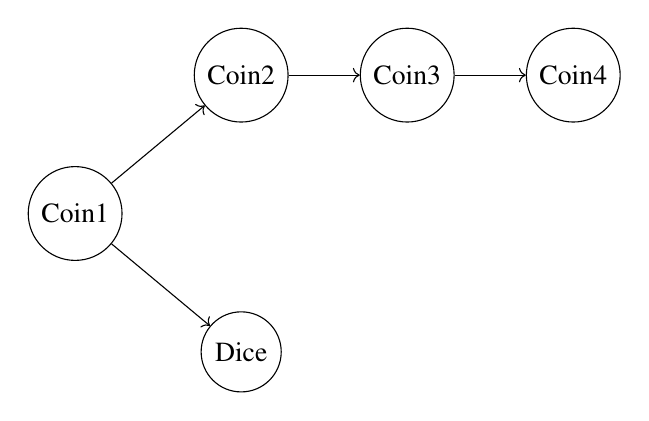
\begin{tikzpicture}
      [sibling distance=10em,level distance=6em, grow=right,
      every node/.style={shape=circle,draw,align=center},->]
      \node{Coin1}
   child
   {
    node{Dice}
   }
   child
   {
    node{Coin2}
      child
      {
        node{Coin3}
        child
      {
        node{Coin4}
      }
      }
    };
\end{tikzpicture}
Let B denote the event that out of last three coins, only one shows tail. \\
By Binomial Distribution,
\begin{align}
\Pr(B)&=\comb{3}{1}\brak{{\dfrac{1}{2}}}^3
\\[\parskip]
&=\dfrac{3}{8}
\end{align}
\\\\
Since tossing a coin and rolling a dice are independent events,
\begin{equation}\label{independent theorem}
\Pr( (X_i=k),(Y=l) )= \Pr(X_i=k)\cdot \Pr(Y=l)
\end{equation}
$k\in\{0,1\}$ and $l\in\{1,2,3,4,5,6\}$.
\\\\
Let A denote the event that the score is 2.
\\\\
Clearly,
\begin{align}
\Pr(A)\nonumber&=\Pr(Y=2|X_1=0)\cdot \Pr(X_1=0) \\
    &+ \Pr(B|X_1=1)\cdot \Pr(X_1=1) 
\\[\parskip]
&=\Pr( (X_1=0),(Y=2) ) + \Pr( (X_1=1), B)
\\[\parskip]
&=\Pr(X_1=0)\cdot \Pr(Y=2)+ \Pr(X_1=1) \cdot \Pr(B)
\\[\parskip]
&=\dfrac{13}{48}
\end{align}
We have to find $\Pr(X_1=0|A)$
\begin{align}
\Pr(X_1=0|A)&=\dfrac{\Pr(A,(X_1=0) )}{\Pr(A)}
\\[\parskip]
&=\dfrac{\Pr(X_1=0)\cdot \Pr(Y=2)}{\Pr(A)}
\\[\parskip]
&=0.31
\end{align}
\\
\textbf{Therefore, required probability = 0.31}
\end{document}
